\documentclass[11pt]{article}
\usepackage[a4paper,left=0.86in,right=0.86in,top=0.86in,bottom=0.96in]{geometry}
\usepackage{amsmath,amssymb,amsthm,mathtools}
\usepackage{graphicx}
\usepackage[hidelinks]{hyperref}
\usepackage{microtype}

\newtheorem{theorem}{Theorem}
\newtheorem{lemma}[theorem]{Lemma}
\newtheorem{remark}[theorem]{Remark}
\newcommand{\F}{\mathbb F_2}
\newcommand{\Z}{\mathbb Z}
\newcommand{\C}{\mathbb C}
\newcommand{\linf}{\ell^\infty}
\newcommand{\Hb}{H_{\!b}}
\newcommand{\eps}{\varepsilon}

\title{The free group algebra \(\ell^1(\mathbb F_2)\)\\
is not ideally amenable}
\author{Candidate full counterexample packet for arXiv:math/0503093}
\date{17 August 2026}

\begin{document}
\maketitle

\begin{abstract}
Let \(q:\mathbb F_2\to\mathbb Z^2\) be abelianization and let \(I\) be the
kernel of the induced quotient homomorphism
\(\ell^1(\mathbb F_2)\to\ell^1(\mathbb Z^2)\).  We construct a non-inner
bounded derivation from \(\ell^1(\mathbb F_2)\) into \(I^*\).  The obstruction
is a scalar bounded two-cocycle coming from an explicit split quasimorphism.
Placing that cocycle in a nonidentity abelianization fiber makes it nonzero in
\(I^\perp\), but zero after inclusion in the full conjugation module
\(\ell^\infty(\mathbb F_2)\).  The resulting connecting class is the required
derivation.  This gives a negative answer to Question~4.4 of the source.
\end{abstract}

\paragraph{Status.}
This is a candidate full proof.  The bounded-cohomology inputs used below are
standard and stated explicitly; the application to the abelianization ideal is
the proposed new step.  No claim is made that the surrounding general
classification problem for \(L^1(G)\) is solved.

\section{The ideal and the coefficient modules}

Put \(G=\F=\langle a\rangle*\langle b\rangle\), \(H=G_{\mathrm{ab}}\cong
\Z^2\), and let \(q:G\to H\) be the quotient map.  The contractive surjective
algebra homomorphism
\[
 Q:\ell^1(G)\longrightarrow\ell^1(H),\qquad
 (Qf)(h)=\sum_{q(g)=h}f(g),
\]
has a closed two-sided kernel \(I\).  Write
\[
 E=\ell^\infty(G)=\ell^1(G)^*,\qquad
 Y=I^\perp=Q^*\ell^\infty(H),\qquad
 X=E/Y\cong I^*.
\]
Thus \(Y\) consists exactly of the functions \(z\circ q\).  Give these spaces
the conjugation action
\begin{equation}\label{eq:conj}
 (g\star F)(x)=F(g^{-1}xg).
\end{equation}
Since \(H\) is abelian, the action on \(Y\cong\ell^\infty(H)\) is trivial.
The sequence
\begin{equation}\label{eq:ses}
 0\longrightarrow Y\xrightarrow{j}E\xrightarrow{p}X\longrightarrow0
\end{equation}
is admissible as a sequence of Banach spaces: a set-theoretic section
\(s:H\to G\) gives the norm-one retraction
\(F\mapsto(h\mapsto F(s(h)))\) of \(j\).

We use inhomogeneous bounded cochains, with
\[
 (\partial\xi)(g)=g\star\xi-\xi,
 \qquad
 (\partial U)(g,h)=g\star U(h)-U(gh)+U(g).
\]

\begin{lemma}[derivations and conjugation cocycles]\label{lem:dictionary}
For every closed ideal \(J\) of \(\ell^1(G)\), bounded derivations
\(D:\ell^1(G)\to J^*\) correspond to bounded one-cocycles
\(b:G\to J^*\) for \eqref{eq:conj}, via
\[
 b(g)=D(\delta_g)\cdot\delta_{g^{-1}},
 \qquad
 D(\delta_g)=b(g)\cdot\delta_g.
\]
Inner derivations correspond exactly to coboundaries.
\end{lemma}

\begin{proof}
The Leibniz rule gives
\[
 b(gh)=b(g)+g\star b(h).
\]
Conversely this identity gives
\(D(\delta_g\delta_h)=\delta_g\cdot D(\delta_h)+
D(\delta_g)\cdot\delta_h\).  Since the module actions of point masses are
isometric and \(b\) is bounded, the formula extends boundedly from point
masses to \(\ell^1(G)\).  Finally,
\(D(\delta_g)=\delta_g\cdot\xi-\xi\cdot\delta_g\) is equivalent to
\(b(g)=g\star\xi-\xi\).
\end{proof}

\section{The cohomological mechanism}

We isolate the only standard bounded-cohomology input.

\begin{lemma}[amenable-stabilizer vanishing]\label{lem:vanish}
If a discrete group \(\Gamma\) acts on a set \(\Omega\) and every point
stabilizer is amenable, then
\[
 \Hb^n(\Gamma,\ell^\infty(\Omega))=0\qquad(n\ge1).
\]
The assertion remains valid for a disjoint union of arbitrarily many orbits.
\end{lemma}

\begin{proof}
For a transitive orbit \(\Gamma/K\), bounded Shapiro identifies the displayed
group with \(\Hb^n(K,\C)\).  Amenability of \(K\) supplies a contracting
homotopy of norm one, hence the latter group vanishes.  The Shapiro maps and
the amenability contraction are norm-controlled independently of the orbit.
For a disjoint union, apply them orbitwise and take the resulting
\(\ell^\infty\)-product; the uniform norm bound makes the combined primitive
bounded.  This is the standard coinduced-module proof of bounded Shapiro and
amenable vanishing \cite[Chs.~7, 10]{Monod}.
\end{proof}

Let
\[
 E_0=\{F\in\ell^\infty(G):F(e)=0\}
     =\ell^\infty(G\setminus\{e\}).
\]
Every nontrivial element of a free group has infinite cyclic centralizer.
The conjugation action on \(G\setminus\{e\}\) therefore has amenable
stabilizers.  Lemma~\ref{lem:vanish} yields
\begin{equation}\label{eq:E0vanish}
 \Hb^n(G,E_0)=0\qquad(n\ge1).
\end{equation}

We now construct the obstruction.  Write each nonidentity element of
\(G=\langle a\rangle*\langle b\rangle\) in reduced syllable form and define
\[
 \varphi(g)=\sum_{\substack{\text{syllables }a^k\\\text{in the reduced form of }g}}
                  \operatorname{sgn}(k),
 \qquad \varphi(e)=0.
\]
When two reduced words are multiplied, fully cancelled syllable pairs make
opposite contributions to \(\varphi\), and at most one final pair of syllables
is merged.  Consequently
\[
 c(g,h):=(\partial\varphi)(g,h)
 =\varphi(g)+\varphi(h)-\varphi(gh)
\]
is bounded (indeed \(|c(g,h)|\le3\)).  Its class in \(\Hb^2(G,\C)\) is
nonzero.  For if \(c=\partial u\) with \(u\) bounded, then
\(\varphi-u\) would be a homomorphism.  But
\[
 \frac{\varphi(a^n)}n\to0,\qquad
 \frac{\varphi(b^n)}n=0,
 \qquad
 \frac{\varphi((ab)^n)}n=1,
\]
which is impossible for a homomorphism at bounded distance from \(\varphi\).

Let \(h_0=(1,0)\in H\), and put \(z=\mathbf1_{\{h_0\}}\in\ell^\infty(H)\).
Because \(Y\) is a trivial \(G\)-module, \(cz\) is a bounded
\(Y\)-valued two-cocycle.  It is not a coboundary: evaluation at \(h_0\) is
an equivariant bounded functional and sends \(cz\) to the nonzero class
\(c\).

On the other hand, the \(E\)-valued cocycle \(j(cz)\) is supported on the
fiber \(q^{-1}(h_0)\), which does not contain \(e\).  It therefore takes values
in \(E_0\), and \eqref{eq:E0vanish} supplies a bounded one-cochain
\(U:G\to E_0\) such that
\begin{equation}\label{eq:primitive}
 \partial U=j(cz).
\end{equation}
Set \(b=pU:G\to X\).  Equation \eqref{eq:primitive} gives
\(\partial b=0\).  Moreover, \(b\) is not a coboundary.  Indeed, if
\(b=\partial\xi\), choose a lift \(\widetilde\xi\in E\) of \(\xi\).  Then
\(U-\partial\widetilde\xi\) is a bounded \(Y\)-valued one-cochain, and its
coboundary is \(j(cz)\).  This would make \(cz\) a coboundary in \(Y\), a
contradiction.  Hence
\begin{equation}\label{eq:nonzero}
 [b]\ne0\quad\text{in}\quad \Hb^1(G,X).
\end{equation}

\section{The counterexample}

\begin{theorem}\label{thm:main}
Let \(I\) be the kernel of the abelianization quotient
\[
 \ell^1(\mathbb F_2)\longrightarrow\ell^1(\mathbb Z^2).
\]
Then
\[
 H^1(\ell^1(\mathbb F_2),I^*)\ne0.
\]
In particular, \(\ell^1(\mathbb F_2)\) is not ideally amenable.
\end{theorem}

\begin{proof}
Identify \(I^*\) with \(X\), and let \(b\) be the nonzero bounded cocycle
from \eqref{eq:nonzero}.  Define first on point masses
\[
 D(\delta_g)=b(g)\cdot\delta_g.
\]
Lemma~\ref{lem:dictionary} extends this to a bounded derivation
\(D:\ell^1(G)\to I^*\).  If \(D\) were inner, the same lemma would make
\(b\) a coboundary, contradicting \eqref{eq:nonzero}.
\end{proof}

\begin{remark}[a wider criterion]
The same proof works for any discrete group \(G\) which has a nontrivial
abelian quotient, amenable centralizers of all nonidentity elements, and
\(\Hb^2(G,\C)\ne0\).  The free group supplies the cleanest instance.
\end{remark}

\clearpage
\section{Source evidence}

The source's page 407 asks explicitly whether \(\ell^1(F_2)\) is ideally
amenable:
\begin{center}
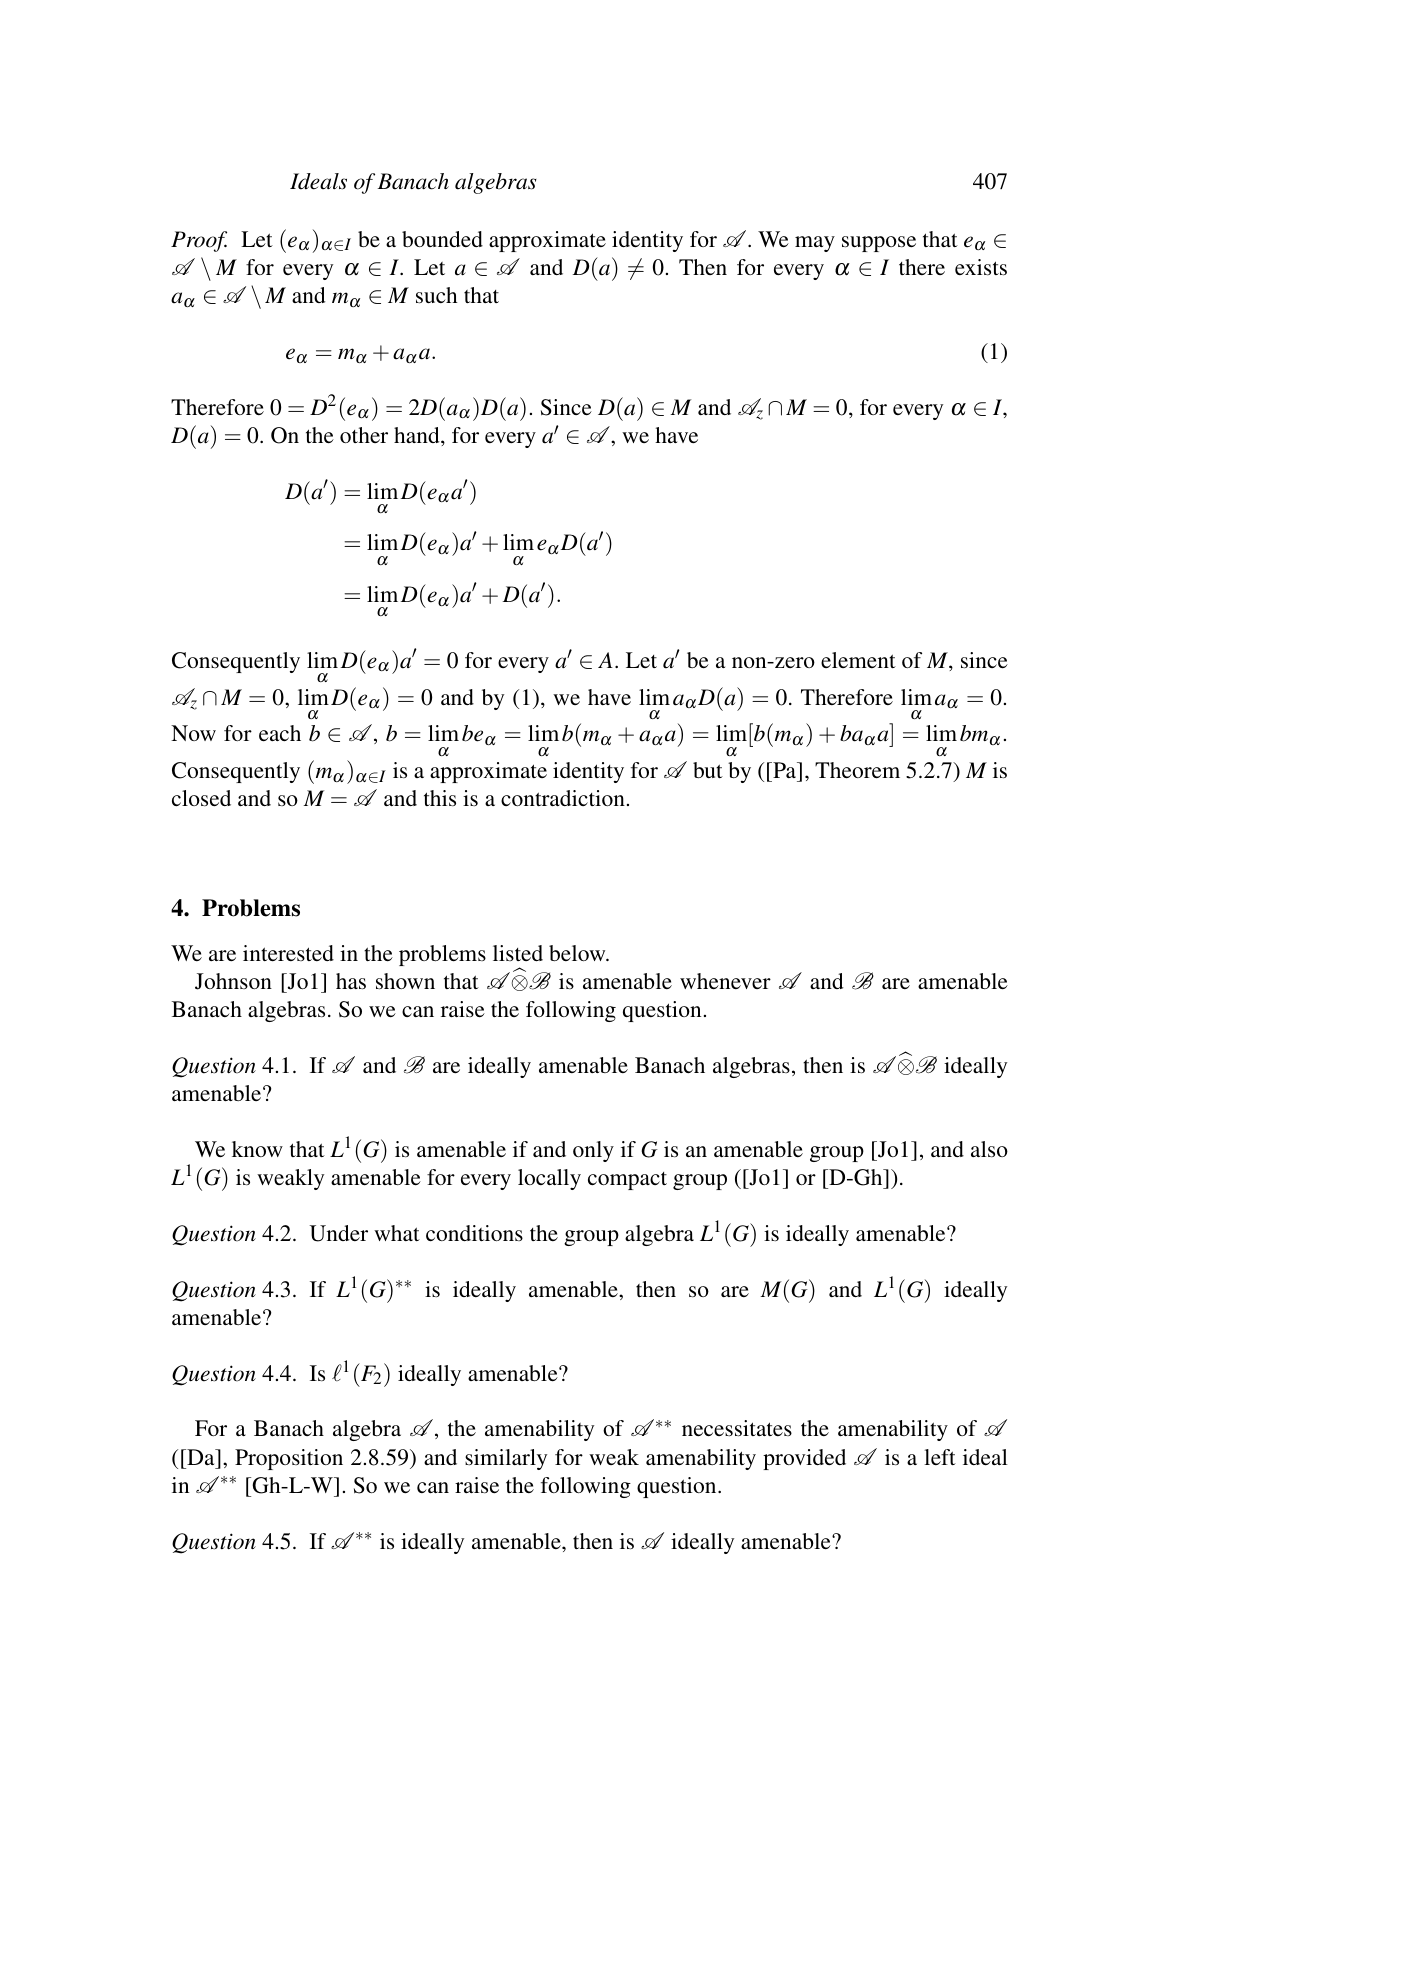
\includegraphics[width=0.91\linewidth,trim=35bp 115bp 35bp 440bp,clip]
 {figures/source_question_page.png}
\end{center}

\begin{thebibliography}{9}
\bibitem{GY}
M.~E.~Gordji and T.~Yazdanpanah,
\emph{Derivations into duals of ideals of Banach algebras},
Proc. Indian Acad. Sci. Math. Sci. \textbf{114} (2004), 399--408;
arXiv:math/0503093.  Question~4.4 is on p.~407.

\bibitem{Monod}
N.~Monod,
\emph{Continuous Bounded Cohomology of Locally Compact Groups},
Lecture Notes in Mathematics 1758, Springer, 2001.
See the bounded Shapiro lemma, relatively injective/coinduced modules, and
amenable vanishing.

\bibitem{GL}
N.~Gr\o nb\ae k and A.~T.-M.~Lau,
\emph{On Hochschild cohomology of the augmentation ideal of a locally compact
group}, Math. Proc. Cambridge Philos. Soc. \textbf{126} (1999), 139--148.
This treats the ordinary augmentation ideal and explains why that ideal alone
does not settle the source question.
\end{thebibliography}

\end{document}
